% Bagian: sets-functions-relations
% Bab: arithmetization
% Subbagian: bilangan real

\documentclass[../../../include/open-logic-section]{subfiles}

\begin{document}

\olfileid[id]{sfr}{arith}{real}
\olsection{Garis Bilangan Real}

Langkah selanjutnya ialah menunjukkan cara membangun bilangan real dari
bilangan rasional. Sebelum itu, kita perlu memahami apa yang
\emph{khas} pada bilangan real.

Bilangan real berperilaku sangat mirip dengan bilangan rasional. (Secara
teknis, keduanya merupakan contoh \emph{lapangan terurut}; untuk definisinya,
lihat \olref[check]{orderedfield}.) Jika Anda telah mengerjakan latihan-latihan
untuk \olref[sfr][siz][]{chap}, Anda akan mengetahui bahwa himpunan bilangan
real mempunyai kardinalitas yang secara ketat lebih besar daripada himpunan
bilangan rasional, yakni $\cardless{\Rat}{\Real}$.
Hal ini pertama kali dibuktikan oleh Cantor. Namun, selama sekitar dua setengah
milenium telah diketahui bahwa ada bilangan irasional, yakni bilangan real yang
bukan bilangan rasional. Bahkan:
%\footnote{Di sini, ``$\sqrt{2}$'' merujuk pada akar kuadrat utama, yakni akar positif.}
\begin{thm}\ollabel{root2irrational}
$\sqrt{2}$ bukan bilangan rasional, yakni $\sqrt{2} \notin \Rat$
\end{thm}

\begin{proof}
Untuk memperoleh kontradiksi, andaikan $\sqrt{2}$ adalah bilangan
rasional. Jadi $\sqrt{2} = \nicefrac{m}{n}$ untuk suatu bilangan asli $m$ dan
$n$. Kita bahkan dapat memilih $m$ dan $n$ sebagai pasangan terkecil yang
mewakili rasio tersebut, sehingga pecahannya tidak dapat disederhanakan lagi.
Dengan menata ulang, $m^{2} = 2n^{2}$. Dari sini, kita
dapat menyelesaikan pembuktian dengan dua cara:

\emph{Pertama, secara geometris} (mengikuti Tennenbaum).\footnote{Bukti ini
dilaporkan oleh \cite{Conway2006}.} Perhatikan persegi-persegi berikut:
\begin{center}	
	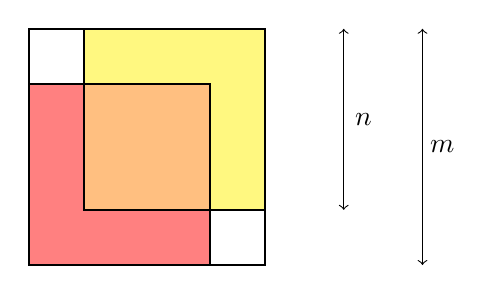
\begin{tikzpicture}
		\draw[thick] (0,0) rectangle (3,3);
		\draw[thick, fill=red!50] (0,0) rectangle (2.3,2.3);
		\draw[thick, fill=yellow!50] (0.7,0.7) rectangle (3, 3);
		\draw[thick, fill=orange!50] (0.7,0.7) rectangle (2.3, 2.3);
		\draw[<->] (4, 0.7)--(4, 3);
		\node at (4.25, 1.85) (n) {$n$};
		\draw[<->] (5, 0)--(5, 3);
		\node at (5.25, 1.5) (m) {$m$};
	\end{tikzpicture}
\end{center}
Karena $m^2 = 2n^2$, daerah tumpang tindih kedua persegi bersisi $n$
mempunyai luas yang sama dengan daerah yang tidak ditutupi oleh kedua
persegi tersebut; yakni, luas persegi jingga sama dengan jumlah luas kedua
persegi yang tidak diarsir. Jadi, jika persegi jingga bersisi $p$ dan setiap
persegi yang tidak diarsir bersisi $q$, maka $p^2 = 2q^2$. Namun, sekarang
$\sqrt{2} = \nicefrac{p}{q}$, dengan $p < m$ dan $q < n$ dan $p, q \in
\Nat$. Hal ini bertentangan dengan fakta bahwa $m$ dan $n$ dipilih sekecil
mungkin.
		
\emph{Kedua, secara formal.} Karena $m^{2} = 2n^{2}$, diperoleh bahwa $m$
genap. (Mudah ditunjukkan bahwa jika $x$ ganjil, maka $x^2$ ganjil.) Jadi
$m = 2r$, untuk suatu $r \in \Nat$. Dengan menata ulang, $2r^2 = n^2$,
		% 				\begin{align*}
		% 					(2q)^{2} &= 2n^{2}\\
		% 					4q^{2} &= 2n^{2}\\
		% 					2q^{2} &= n^{2}
		% 				\end{align*}
maka $n$ juga genap. Jadi $m$ dan $n$ keduanya genap, sehingga pecahan
$\nicefrac{m}{n}$ \emph{dapat} disederhanakan lagi. Kontradiksi!
\end{proof}

Sambil lalu, bukti diagramatis ini memungkinkan kita meninjau kembali materi dari
\olref[his][set][mythology]{sec}. Tennenbaum (1927--2006) adalah seorang
matematikawan yang sepenuhnya modern; tetapi bukti tersebut tidak dapat disangkal keindahannya,
sepenuhnya ketat secara matematis, dan menggunakan intuisi geometris!

Bagaimanapun, bilangan real ``lebih luas'' daripada bilangan rasional. Dalam
arti tertentu, terdapat ``celah-celah'' pada bilangan rasional, dan celah-celah
ini diisi oleh bilangan real. Weierstrass menyadari bahwa hal ini menggambarkan
satu sifat bilangan real yang membedakannya dari bilangan rasional, yakni Sifat
Kelengkapan: \emph{Setiap himpunan takkosong bilangan real yang mempunyai suatu
batas atas mempunyai suatu batas atas terkecil.}

Mudah dilihat bahwa bilangan rasional tidak memiliki Sifat Kelengkapan. Sebagai
contoh, perhatikan himpunan bilangan rasional yang lebih kecil daripada
$\sqrt{2}$, yakni:
\[
	\Setabs{p \in \Rat}{p^2 < 2 \text{ atau }p < 0}
\]
Himpunan ini mempunyai suatu batas atas dalam bilangan rasional; sebagai
contoh, semua !!{element}s< himpunan ini lebih kecil daripada $3$. Namun, apa
batas atas terkecilnya? Kita ingin mengatakan `$\sqrt{2}$'; tetapi kita baru
saja melihat bahwa $\sqrt{2}$ \emph{bukan} bilangan rasional. Tidak ada pula
bilangan rasional \emph{terkecil} yang lebih besar daripada $\sqrt{2}$. Jadi,
himpunan tersebut mempunyai suatu batas atas tetapi tidak mempunyai batas atas
terkecil. Oleh karena itu, bilangan rasional tidak memiliki Sifat Kelengkapan.

Sebaliknya, kontinuum ``secara moral semestinya'' memiliki Sifat Kelengkapan.
Kita tidak hanya menginginkan $\sqrt{2}$ menjadi bilangan real; kita ingin
mengisi semua ``celah'' pada garis bilangan rasional. Bahkan, kita ingin
kontinuum itu sendiri tidak memiliki ``celah''. Itulah tepatnya yang akan kita
peroleh melalui Kelengkapan.

\end{document}
